% Replaces the experiments section from the RD figure to the end of "Codec design choices".
% Preamble: \newcommand{\MSc}{MeshSplatting-cap\xspace}
%------------------------------------------------------------------
\begin{figure*}[t]\centering
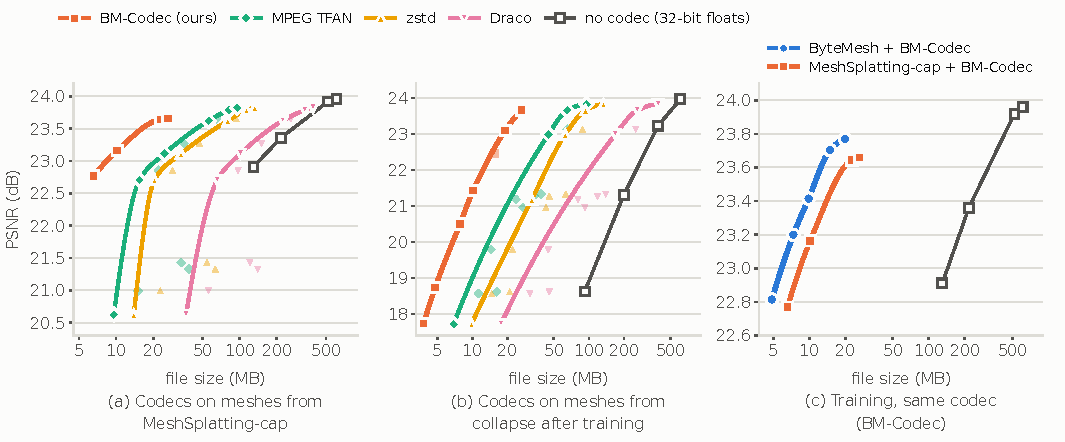
\includegraphics[width=\linewidth]{figures/fig_rd_three_v6.pdf}
\caption{\textbf{Rate--distortion on Mip-NeRF~360 and Tanks and Temples} (mean over 11 scenes). (a)~Meshes from \MSc, written by BM-Codec and by the baseline codecs. (b)~The same comparison on meshes from collapse after training. (c)~Meshes from \BM and from \MSc, both written by BM-Codec. The grey line is the meshes from \MSc (a, c) or from collapse after training (b) without a codec. The panels have different PSNR ranges.}
\label{fig:rd}
\end{figure*}

\begin{table}[t]\centering\footnotesize
\caption{\textbf{BD-rate of each codec relative to the same meshes without a codec} (32-bit floats). Meshes from \MSc; computed per scene and averaged over each dataset. More negative is better.}
\label{tab:bd}
\setlength{\tabcolsep}{4pt}
\begin{tabular}{@{}lccc@{}}
\toprule
 & Mip-NeRF 360, & Deep & NeRF- \\
codec & T\&T (11) & Blending (2) & Synthetic (8) \\
\midrule
Draco & $-27.3\%$ & $-11.3\%$ & $-9.7\%$ \\
zstd & $-76.0\%$ & $-75.0\%$ & $-78.5\%$ \\
MPEG TFAN & $-82.5\%$ & $-82.3\%$ & $-83.0\%$ \\
BM-Codec (ours) & $\mathbf{-93.6\%}$ & $\mathbf{-93.4\%}$ & $\mathbf{-88.9\%}$ \\
\bottomrule
\end{tabular}
\end{table}
%------------------------------------------------------------------

\subsection{Codec efficiency}
\label{sec:codec}
We first evaluate BM-Codec alone (Fig.~\ref{fig:rd}a). For each scene, we train \MSc with three caps and \MS with its default cap, which gives four meshes per scene (three per object on NeRF-Synthetic). On Mip-NeRF~360 and Tanks and Temples the caps are 0.6, 1.08, 3 and 4 million vertices. The grey line in Fig.~\ref{fig:rd}a shows these meshes before coding, stored in 32-bit floats (130 to 609~MB on these two datasets). BM-Codec writes each mesh into one file, which gives one point per mesh. A baseline codec is run with three SH precisions, which gives three points per mesh. Each point in Fig.~\ref{fig:rd}a is the mean over the 11 scenes for one cap and one precision. All codecs see the same meshes, so only the codec differs.

Table~\ref{tab:bd} gives the BD-rate of each codec relative to the same meshes without a codec. On Mip-NeRF~360 and Tanks and Temples, BM-Codec removes 93.6\% of the bytes at the same PSNR. TFAN removes 82.5\%, zstd 76.0\% and Draco 27.3\%. Compared directly on these two datasets, BM-Codec needs 63\% fewer bytes than TFAN, 73\% fewer than zstd and 91\% fewer than Draco at the same PSNR. Deep Blending gives similar numbers. On NeRF-Synthetic, BM-Codec removes 88.9\% of the bytes and TFAN 83.0\%. The rate--distortion curves on Deep Blending and NeRF-Synthetic are in the supplement.

BM-Codec is lossy. On the 11 scenes of Mip-NeRF~360 and Tanks and Temples, its lossy steps (vector quantization of the SH coefficients and quantization of positions and color) lower the PSNR by 0.15 to 0.27\dB on average, relative to the same meshes before coding.

\subsection{Collapse after training}
\label{sec:simp}
We repeat the comparison on a second set of meshes, on the same 11 scenes. These meshes are obtained by reducing the FP32 model with edge collapse after training (Fig.~\ref{fig:rd}b). The order of the codecs is the same. Relative to these meshes without a codec, BM-Codec removes 95.1\% of the bytes at the same PSNR. TFAN removes 87.5\%, zstd 81.8\% and Draco 56.0\%. The gain of BM-Codec therefore does not depend on how the meshes were obtained.

These meshes are, however, much worse than those of \MSc. We compare the two at the same vertex count on all 21 scenes, with several vertex counts per scene (128 pairs in total). \MSc is better on 127 of the 128 pairs, by 1.86\dB on average. The loss grows as the mesh is reduced. The reason is that each pixel is covered by one opaque triangle. After a collapse, the neighboring triangles have not been trained for their new shape, and no other primitive covers the error. We therefore use \MSc as the baseline for the training in the next section. Fig.~\ref{fig:qual} shows the three ways to reach the same file size on three scenes.

\subsection{Gain of rate-controlled training}
\label{sec:rd}
We now fix the codec to BM-Codec and evaluate the gain from rate-controlled training (\BM) compared to MeshSplatting training using different vertex caps (Fig.~\ref{fig:rd}c). Table~\ref{tab:bd-train} gives the Bjontegaard deltas for each dataset. \BM is better than \MSc on 20 of the 21 scenes and equal on one (treehill). Over the 21 scenes, the BD-PSNR is $+0.29$\dB on average and the BD-rate is $-26.9\%$.

\begin{table}[t]\centering\footnotesize
\caption{\textbf{Gain of rate-controlled training}: Bjontegaard deltas of \BM against \MSc, both written by BM-Codec, computed per scene and averaged over each dataset.}
\label{tab:bd-train}
\begin{tabular}{@{}lcc@{}}
\toprule
dataset (scenes) & BD-PSNR & BD-rate \\
\midrule
Mip-NeRF 360, T\&T (11) & $+0.30$ dB & $-31.3\%$ \\
Deep Blending (2) & $+0.23$ dB & $-22.8\%$ \\
NeRF-Synthetic (8) & $+0.29$ dB & $-21.1\%$ \\
all (21) & $+0.29$ dB & $-26.9\%$ \\
\bottomrule
\end{tabular}
\end{table}

\begin{table}[t]\centering\footnotesize
\caption{\textbf{\BM at three target sizes and the FP32 model of \MS}, dataset means over single runs; size in MB. Size error is $|\text{file}-\text{target}|/\text{target}$. All targets are in the supplement. $^\dagger$Two objects (ficus, mic) are fully represented by about 2 to 2.6~MB and do not grow further.}
\label{tab:main}
\setlength{\tabcolsep}{3.2pt}
\begin{tabular}{@{}llccccc@{}}
\toprule
dataset & target & size & err. & PSNR & SSIM & LPIPS \\
\midrule
\multirow{4}{*}{\shortstack[l]{Mip-NeRF\\360 (9)}} & 20 & 19.91 & 0.8\% & 24.46 & 0.707 & 0.406 \\
 & 10 & 9.87 & 1.5\% & 24.06 & 0.678 & 0.453 \\
 & 5 & 4.85 & 2.9\% & 23.42 & 0.635 & 0.506 \\
 & FP32 & 642 & -- & 24.81 & 0.731 & 0.309 \\
\midrule
\multirow{4}{*}{\shortstack[l]{Tanks and\\Temples (2)}} & 20 & 20.01 & 0.2\% & 20.64 & 0.750 & 0.332 \\
 & 10 & 9.94 & 0.6\% & 20.51 & 0.736 & 0.361 \\
 & 5 & 4.96 & 0.8\% & 20.09 & 0.703 & 0.408 \\
 & FP32 & 459 & -- & 20.64 & 0.760 & 0.272 \\
\midrule
\multirow{4}{*}{\shortstack[l]{Deep\\Blending (2)}} & 20 & 19.93 & 0.9\% & 27.01 & 0.840 & 0.450 \\
 & 10 & 9.93 & 0.7\% & 26.69 & 0.833 & 0.474 \\
 & 5 & 4.99 & 0.3\% & 26.04 & 0.821 & 0.498 \\
 & FP32 & 772 & -- & 27.23 & 0.842 & 0.337 \\
\midrule
\multirow{4}{*}{\shortstack[l]{NeRF-\\Synthetic (8)}} & 4$^\dagger$ & 3.56 & 11.3\% & 31.20 & 0.952 & 0.069 \\
 & 2.5$^\dagger$ & 2.43 & 3.2\% & 31.10 & 0.951 & 0.069 \\
 & 1.5 & 1.50 & 0.3\% & 30.45 & 0.945 & 0.079 \\
 & FP32 & 65.7 & -- & 31.17 & 0.955 & 0.063 \\
\bottomrule
\end{tabular}
\end{table}

\noindent\textbf{Against the FP32 model.} At the highest target of 20~MB, the files of \BM are 31 times smaller than the FP32 model on Mip-NeRF~360 and Tanks and Temples (609~MB on average over the 11 scenes), for a PSNR loss of 0.28\dB. On NeRF-Synthetic, the 3.6~MB files match the PSNR of the 65.7~MB FP32 models (mean over the 8 objects).

\subsubsection{File Size Control Effectiveness}
With \MSc, the same cap gives files of very different sizes. Over the 13 scenes of Mip-NeRF~360, Tanks and Temples and Deep Blending, the files range from 5.8 to 7.5~MB at a cap of 0.6 million vertices, and from 20.0 to 39.8~MB at the default cap of 4 million (supplement). The cap for a desired file size therefore depends on the scene. \BM takes the file size as its input and progressively updates the vertex count based on the encoding results from previous iterations; it can reach the target size within a small margin without requiring prior knowledge of the scene. Table~\ref{tab:main} lists its results. On these 13 scenes, at five targets from 5 to 20~MB, all 65 runs end within 10\% of the target, and the mean size error is 1.3\%. On the 8 objects of NeRF-Synthetic, at three targets from 1.5 to 4~MB, 21 of 24 runs end within 10\%. The three other runs are ficus and mic at 2.5 or 4~MB. These two objects are fully represented by about 2 to 2.6~MB, so the file stays below the target.

\subsection{Other representations}
\label{sec:cross}

\begin{table}[t]\centering\footnotesize
\caption{\textbf{Other representations on Mip-NeRF~360}; size in MB. Gaussian rows are published numbers collected in~\cite{hacpp2025} and are given for reference. Mesh rows are published numbers collected in~\cite{meshsplatting2025}. \MS FP32 is our reproduction.}
\label{tab:cross}
\setlength{\tabcolsep}{4pt}
\begin{tabular}{@{}lcccc@{}}
\toprule
method & PSNR & SSIM & LPIPS & MB \\
\midrule
3DGS~\cite{kerbl2023gaussians} & 27.46 & 0.812 & 0.222 & 750.9 \\
Compact3DGS~\cite{compact3dgs2024} & 27.08 & 0.798 & 0.247 & 48.80 \\
HAC++~\cite{hacpp2025}, low & 27.60 & 0.803 & 0.253 & 8.34 \\
HAC++, high & 27.82 & 0.811 & 0.231 & 18.48 \\
\midrule
GOF mesh~\cite{gof2024} & 20.78 & 0.573 & 0.465 & 1500 \\
RaDe-GS mesh~\cite{rade2024} & 23.56 & 0.668 & 0.361 & 1100 \\
MiLo~\cite{milo2025} & 24.09 & 0.688 & 0.323 & 253 \\
\MS FP32~\cite{meshsplatting2025} & 24.81 & 0.731 & 0.309 & 642 \\
\midrule
\BM, 20 MB & 24.46 & 0.707 & 0.406 & 19.9 \\
\BM, 10 MB & 24.06 & 0.678 & 0.453 & 9.9 \\
\BM, 5 MB & 23.42 & 0.635 & 0.506 & 4.9 \\
\bottomrule
\end{tabular}
\end{table}

Table~\ref{tab:cross} compares \BM with other representations on the 9 scenes of Mip-NeRF~360. Among the methods that output a mesh, \BM is the only one below 20~MB. At 20~MB it is 0.35\dB below the FP32 model of \MS, and it is above MiLo, RaDe-GS and GOF with files 13 to 75 times smaller. Compressed Gaussians remain better at the same size: HAC++ is 3.4 to 4.2\dB higher in PSNR. This gap comes from the representation (opaque triangles against semi-transparent Gaussians) and is already present before compression, between \MS and 3DGS. What the mesh offers in exchange is a standard indexed triangle mesh that any engine renders without sorting. We measured the rendering time of our meshes in a WebGL viewer on a laptop (Apple M2 Max, $1920 \times 958$). The 5, 10 and 20~MB files of \BM for garden, room and bicycle take 1.1, 1.3 and 2.0~ms per frame on average over the three scenes. In the same viewer, the FP32 meshes of \MS for garden and bicycle take 19.3 and 13.1~ms per frame.

\subsection{Complexity}
\label{sec:time}

\begin{table}[t]\centering\footnotesize
\caption{\textbf{File size, quality and coding time} on the same meshes: \MSc with a cap of about 1.08 million vertices, mean over the 11 scenes of Mip-NeRF~360 and Tanks and Temples. The baseline codecs use 8-bit SH coefficients. Times in seconds. The vector quantization of BM-Codec runs on a GPU; everything else runs on a CPU. TFAN was timed in a separate run on another node.}
\label{tab:time}
\setlength{\tabcolsep}{3.6pt}
\begin{tabular}{@{}lcccc@{}}
\toprule
codec & MB & PSNR & encode & decode \\
\midrule
no codec (32-bit floats) & 216 & 23.36 & -- & -- \\
Draco & 150.9 & 23.27 & 16.6 & 3.8 \\
zstd (quantized PLY) & 47.3 & 23.27 & 15.4 & 0.2 \\
MPEG TFAN & 35.6 & 23.27 & 6.4 & 2.8 \\
\midrule
BM-Codec & 10.2 & 23.16 & 60.7 & 3.7 \\
% BM-Codec, no refinement & ?? & ?? & 12.9 & 3.7 \\   % size and PSNR: from vq-noref.txt (batch45), then uncomment
\bottomrule
\end{tabular}
\end{table}

Table~\ref{tab:time} gives the file size, the PSNR and the coding times of each codec on the same meshes. The encoding of BM-Codec has four steps. $k$-means builds the two codebooks on 65{,}536 sampled vertices (2.6~s). Every vertex is then assigned its nearest codeword in each codebook (5.7~s). The codewords are refined for 400 steps on the rendering loss, with the indices fixed (47.7~s). The entropy coding writes the file (4.6~s). The refinement takes most of the time, because every step renders images. It halves the loss of the vector quantization: on the validation views of these 11 scenes, the loss is 0.48\dB on average after $k$-means alone and 0.24\dB after the refinement. In total, encoding takes about one minute and is slower than the baseline codecs. Decoding takes 3.7 seconds, similar to Draco and TFAN. One training run of \BM takes 48.8 minutes on average over the 13 scenes of Mip-NeRF~360, Tanks and Temples and Deep Blending (one L40S GPU), including the size probes.

\subsection{Ablation}
\label{sec:abl}

\begin{table}[t]\centering\footnotesize
\caption{\textbf{Selection rules}: PSNR change (dB) when the split rule or the collapse rule is replaced by the importance score of \MS. Five scenes of Mip-NeRF~360 and Tanks and Temples, target 10~MB, one run each; every file is within 3\% of the target.}
\label{tab:abl}
\setlength{\tabcolsep}{3.2pt}
\begin{tabular}{@{}lcccccc@{}}
\toprule
 & garden & room & bicycle & kitchen & truck & mean \\
\midrule
split by importance & $-0.17$ & $-0.43$ & $-0.29$ & $-0.62$ & $-0.20$ & $-0.34$ \\
collapse by importance & $-0.78$ & $-2.38$ & $-0.08$ & $-5.68$ & $-0.69$ & $-1.92$ \\
\bottomrule
\end{tabular}
\end{table}

\noindent\textbf{Selection rules.} \BM uses the per-triangle error $e_t$ in both rules: it splits the triangles with the largest error, and collapses the edges with the least error per byte saved. Table~\ref{tab:abl} replaces $e_t$ in one rule at a time by the importance score that \MS computes for each triangle, and keeps everything else. We test five scenes at a target of 10~MB. Both replacements lower the PSNR on all five scenes. The mean loss over the five scenes is 0.34\dB for the split rule and 1.92\dB for the collapse rule.

\begin{table}[t]\centering\footnotesize
\caption{\textbf{Effect of the growth aim $\alpha$} on two scenes of Mip-NeRF~360. Target 10~MB, one run each.}
\label{tab:alpha}
\setlength{\tabcolsep}{5pt}
\begin{tabular}{@{}lcccc@{}}
\toprule
 & \multicolumn{2}{c}{garden} & \multicolumn{2}{c}{room} \\
\cmidrule(lr){2-3}\cmidrule(lr){4-5}
$\alpha$ & size (MB) & PSNR (dB) & size (MB) & PSNR (dB) \\
\midrule
1.0 & 8.46 & 23.33 & 8.72 & 27.65 \\
1.2 & 9.94 & 23.57 & 10.03 & 27.90 \\
1.35 & 10.00 & 23.67 & 9.99 & 27.99 \\
1.5 & 9.96 & 23.76 & 9.70 & 27.84 \\
\bottomrule
\end{tabular}
\end{table}

\noindent\textbf{Growth aim.} \BM grows the mesh to $\alpha = 1.35$ times the target and then removes the excess. Table~\ref{tab:alpha} varies $\alpha$ on garden and room at a target of 10~MB. With $\alpha = 1.0$, the file ends 15\% below the target on garden and 13\% below on room, and no collapse round is active: vertices are lost between the end of densification and the triangulation, and nothing can add them back. Growing past the target is therefore necessary. Between 1.2 and 1.5, the file is within 3\% of the target on both scenes and the PSNR changes by less than 0.2\dB. We use $\alpha = 1.35$ for all scenes.

\begin{table}[t]\centering\footnotesize
\caption{\textbf{Codec design choices}, mean over the 11 scenes of Mip-NeRF~360 and Tanks and Temples (meshes of about one million vertices). The first row of each block is the codec used for all other results.}
\label{tab:codec-abl}
\setlength{\tabcolsep}{4pt}
\begin{tabular}{@{}llcc@{}}
\toprule
attribute & coding method & bits/vertex & size change \\
\midrule
\multirow{4}{*}{positions} & one earlier neighbor & 22.6 & -- \\
 & previous vertex & 23.2 & $+0.7\%$ \\
 & parallelogram & 23.5 & $+1.0\%$ \\
 & mean of earlier neighbors & 21.6 & $-1.1\%$ \\
\midrule
\multirow{2}{*}{DC color} & zstd, no prediction & 12.6 & -- \\
 & mean of earlier neighbors & 11.3 & $-1.5\%$ \\
\midrule
\multirow{3}{*}{SH indices} & earlier neighbors as candidates & 17.6 & -- \\
 & no neighbor information & 17.4 & $-0.3\%$ \\
 & fixed length & 20.0 & $+2.8\%$ \\
\bottomrule
\end{tabular}
\end{table}

\noindent\textbf{Codec design choices.} Table~\ref{tab:codec-abl} measures alternatives for the lossless coding of three vertex attributes on the same meshes of these 11 scenes. For positions, BM-Codec predicts a vertex from one earlier neighbor: among the connected vertices that are already decoded, the one with the smallest index. The decoder finds it from the connectivity, so no bits are spent on the choice. On all 11 scenes, this gives a smaller stream than prediction from the previously coded vertex and than parallelogram prediction. Predicting from the mean of all earlier connected neighbors is better still, and the same holds for the DC color. For the SH indices, BM-Codec offers the indices of the earlier connected neighbors as candidates. This does not help: coding each index directly with an arithmetic coder, whose symbol probabilities are updated as the indices are coded, gives slightly smaller streams. Together, the better variants would make the files about 2.9\% smaller on average over the 11 scenes. They are not used in the reported results, so the reported sizes are conservative.
